\section{Digital Image Processing}
Digital image processing is a wide research field with many subspecialities.
Gonzalez and Woods \cite{gonzalez2008} goes in their book through some of them.
From image representation to transformations, filtering, restoriation and finishes
of with compression, segmentation and recognition. To be able to better grasp
the image segmentation algorithm in the following chapters some basics will be
explained first.

\subsection{Digital image representation}
To be able to present, transfer and alter a digital image we first need someway
to represent it on a computer. This is generally done by dividing an image into
its smallest part, {\em pixels}. Each pixel holds a value that defines its {\em intensity}.
The simplest kind of image is a binary-image. Each pixel has a value of either
0 or 1, where 0 means no intensity and 1 means maximum intensity. A more common
description of such an image is a black and white image where 0 means black and
1 means white.

When more colors are needed the intensity span is increased to give room for more
variation. This is often in the size of 8-bits, 0 to 255. Where 0 means no intensity
and 255 maximum intensity. A gray-scale image would be described in this way; one 8-bit
{\em channel}, 0 as black, 255 as white and everything inbetween is gray.
To be able to represent a color image more channels are needed. One common way
to describe color images is the RGB color space. R for red, G for green and B for
blue.

\begin{figure}[ht]
    \begin{minipage}[t]{0.45\linewidth}
        \centering
        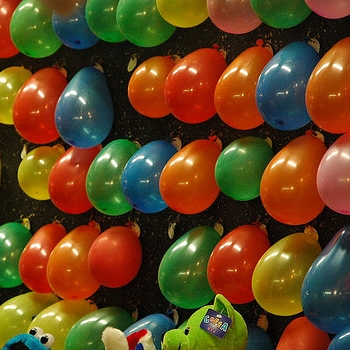
\includegraphics[width=\textwidth]{images/balloons/balloons-original.jpg}
        \caption{Balloons, RGB color image \cite{balloons}.}
        \label{fig:balloons-rgb}
    \end{minipage}
    \hspace{0.5cm}
    \begin{minipage}[t]{0.45\linewidth}
        \centering
        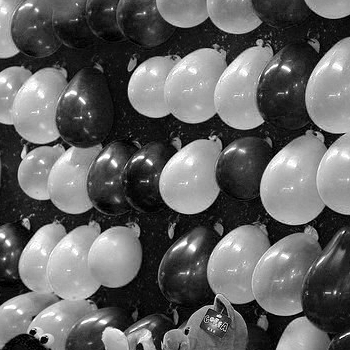
\includegraphics[width=\textwidth]{images/balloons/balloons-red-channel.jpg}
        \caption{Balloons, red channel \cite{balloons}.}
        \label{fig:balloons-red}
    \end{minipage}
\end{figure}
\begin{figure}[ht]
    \begin{minipage}[t]{0.45\linewidth}
        \centering
        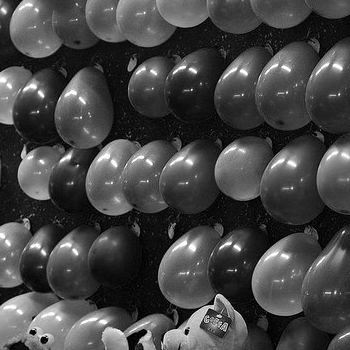
\includegraphics[width=\textwidth]{images/balloons/balloons-green-channel.jpg}
        \caption{Balloons, green channel \cite{balloons}.}
        \label{fig:balloons-green}
    \end{minipage}
    \hspace{0.5cm}
    \begin{minipage}[t]{0.45\linewidth}
        \centering
        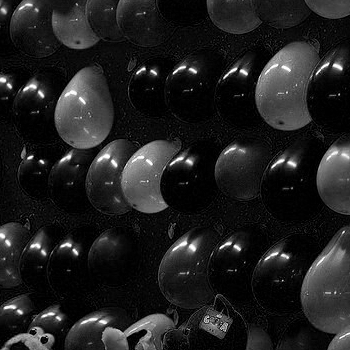
\includegraphics[width=\textwidth]{images/balloons/balloons-blue-channel.jpg}
        \caption{Balloons, blue channel \cite{balloons}.}
        \label{fig:balloons-blue}
    \end{minipage}
\end{figure}

An example to this can be seen in figures \ref{fig:balloons-rgb},
\ref{fig:balloons-red}, \ref{fig:balloons-green} and \ref{fig:balloons-blue}.
Figure \ref{fig:balloons-rgb} is the original in RGB color. Figure \ref{fig:balloons-red},
\ref{fig:balloons-green} and \ref{fig:balloons-blue} represent the intensity in the red,
green and blue channel respectively. A region in an image that is white (high
intensity) in all three channels is white in the RGB original as well, this can
be seen in the lower left as the eyeballs of the cuddly toy. A region that is white
in red channel and black in the blue and green channel is red in the RGB original, as
can be seen for all red balloons.

Though looking at only two channels can not tell the entire truth. As an example all
yellow balloons could be interpreted as red ballons if you only look at the
red and blue channels. The only difference between red and yellow balloons is
seen in the green channel where the intensity of yellow balloons is higher than
there red counterparts.

The RGB color space is one of the standard color models used today, other models
worth mentioning is the CMY (or CMYK) and HSI color model. These color space
models are out of scope of this report. For more information about them,
reading chapter 6 of "Digital image processing" by Gonzalez and Woods \cite{gonzalez2008} is suggested.

As an image always is two dimensional it's common to describe its intensity as
a function of x and y coordinates (Eq. \ref{eq:intensity}). The indexing of
rows and columns starts in the upper left corner with element (0,0) and increases
in x direction downwards and in y direction to the right. As an example if an
image has 100 pixels in a square the bottom right pixel will be indexed (10,10) \cite{gonzalez2008}.
\begin{equation}
    \label{eq:intensity}
    I(x,y)
\end{equation}

\subsection{Filtering and Gaussian smoothing}
An image's quality depends on a lot of factors. During aquisition some kind of
camera is used, first of all the quality of the image depends on the quality
of the camera. The lens and sensor needs to be adequate for its usage.
It also depends on how the image is stored, many mobile phone cameras store
the images in compressed format and there is no way to get the uncompressed
image back. Independent of how an image is aquired the image will always have
some artifacts, or in another term, some noise in it. This noise can be described
as a part of the image that is displayed on a computer. From equation \ref{eq:intensity}
 the true intensity from a pixel is given and the noise is added to it as \(n(x,y)\) in
 equation \ref{eq:intensityNoise}, the result is the image as it's displayed. In other
 terms the image that you view on a computer is never perfect, it always has some
 noise or artifacts in it.
\begin{equation}
    \label{eq:intensityNoise}
    \hat{I}(x,y) = I(x,y) + n(x,y)
\end{equation}

The problem to remove as much noise as possible but still keep key features of
an image is a big problem. The reason for this is that noise can be described
as a high variation in intensity between neighbouring pixels and the exact
same description can be used for describing edges between different regions
in an image.

% 0. The purpose to remove artifacts.
% 1. Start with statistics normal distribution and standard deviation.
% 2. Continue with one dimensional example.
% 3. Move to 2 dimensional
% 4. Introduce the kernel and apply it to some image (smile)

\subsection{Image segmentation}
A big part of digital image processing is taking an image, modify it and
return a new image. Image segmentation is instead taking an image as input,
identifying interesting regions and return thoose regions back to the user.
This could be done for detecting veins and arteries in medical images \cite{olena2010},
for detecting objects moving across a road or identifying missing components on
a circuit board in a factory during the certification process in the end of a production line.
Image segmentation is a main step before object recognition can be made.

The most basic image segmentation methods try to identify points, lines and edges
and work from there.

% TODO: Can add mathematical details about isolated point detection.
